% example of how to use template

% set the template of document
\documentclass[natbib]{muthesis}
\usepackage{graphicx}
\usepackage{url}
\usepackage{float}
\usepackage{subfig}
\usepackage{etoolbox}
\usepackage{mathtools,amsmath}
\usepackage{physics}
\usepackage{empheq}
\usepackage{esdiff}
\restylefloat{table}
\restylefloat{figure}
\usepackage{caption}
\bibliographystyle{plain} % if you are using bibtex
\graphicspath{ {./images/} }

% create new command for convenience
% \newcommand{\beq}{\begin{equation}}
% \newcommand{\eeq}{\end{equation}}
% \newcommand{\bfig}{\begin{figure}}
% \newcommand{\efig}{\end{figure}}
% \newcommand{\bfa}{\left\{\begin{array}}
% \newcommand{\efa}{\end{array}\right.}
% \renewcommand{\arraystretch}{1.5}

% set number of candidate (from 1 - 3) and advisor (from 1 - 2)
\noofcandidate{1}
\noofadvisor{1}

% information for front page
\title{Automatic Subtitle Generator}
\candidate{Aphisit Areechitsakul}

\degree{B.Sc.}
\subject{Computer Science}
\submissionyear{2020}

% information for page i (advisors)
\candidatetitle{}
\majoradvisor{Dr.Sunsern Cheamanunkul}
\majoradvisorsubject{Computer Science}

% information for page ii (exam committee)
\submissiondate{8th April 2020}

% Advisor
\advisor{Dr.Sunsern Cheamanunkul}

% Program Director
\programdirector{Dr. Kritya Bunchongchit}
% Division Chair
\chair{Assoc. Prof. Dr. Pakorn Bovonsombat}

% information for page iv (ABSTRACT)

\candidatenumber{5880685 ICCS/B}

%\longsubject
\keywords{speech recognition, word error rate}

% information for biography

% For first candidate
\dateofbirth{8th November 1997}
\placeofbirth{Samut Sakhon , Thailand}
\firstdegree{IGCSE}
\firstdegreemajor{Grade 11}
\firstdegreeinstitution{Traill International School}
\firstdegreeyears{2010-2013}
\years{2014-2019}
\homeaddress{51/7 moo 3 Soi Ekkachai 147 Ekkachai Road}
\homeaddressLnII{T. Bangnamjeud A.Muang}
\homeaddressLnIII{Samut Sakhon, 74000, Thailand}
\email{bright40081@n@gmail.com}

\begin{document}

  \maketitle

  \acknowledgements{
	I would like to express my thanks of gratitude to my advisor Dr.Sunsern Cheamanunkul, and other professors at MUIC who given me the knowledge during my college years on campus. I also would like to thank my family and friends for their support and encouragement throughout my whole journey.
  }

  \abstract{
  	
  }

  % Table of content
  \linespacing{1.2}
  \tableofcontents

  \linespacing{1.77}

% \cite{name}
% ------ Chapter 1 -------
  \chapter{Introduction}
  \section{Motivation}
  Video is one of the popular media that people can easily access and watch it for various purposes, such as education and entertainment. Nevertheless, many of us cannot fully understand the content of video due to language barrier. As such, subtitle can play an important role to help us understand more about the part of content that we missed. It also help us to feel familiar with the accent and pronunciation, which allows us to improve our language skills better. Moreover, having subtitles gives the opportunity to deaf people enjoy videos. Deaf people normally watch the videos with either sign languages or subtitles, but not all videos come with them, especially lecturing and recording video type. 
  
  %---change to 2 point---
  \section{Objective}
  The goal of this project is to implement the automatic subtitle generator service by making use of the existing speech recognition services and open-sources, including Amazon Transcribe, CMUSphinx, DeepSpeech and Google Web Speech, together with evaluating the performance of each speech recognition system.
  
  \section{Timeline}
  gant chart
  
  % ------ Chapter 2 -------
  \chapter{Literature Review}
  
  \section{Exisiting Solutions}
  %slide
  
  \section{Overview of Automatic Speech Recognition}
  
  \begin{figure}[H]
  	\centering
  	\captionsetup{justification=centering}
  	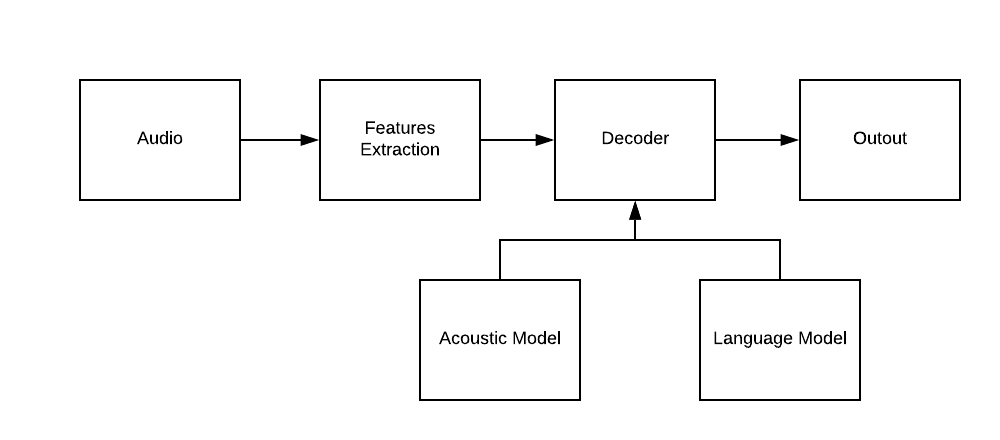
\includegraphics[width=0.9\linewidth]{images/traditional-asr}
  	\caption{Traditional ASR pipeline}
  	\label{fig:traditional-asr}
  \end{figure}
  Automatic Speech Recognition(ASR) is a technology that allows the computer to identify human spoken words and convert them into the digital text. The main components in ASR are acoustic and language models.
  Figure 2.1 illustrate the flow of traditional automatic speech recognition for transcribing.
  Firstly, It takes in the audio wave as an input and extract its features in preprocessing step. During the decoding part, the system used acoustic model to recognize the phonetics from data representation and decode them through the language model to produce the proper text. 
  
  Originally, the acoustic model is trained by using Gaussian Mixture Model(GMM) based Hidden Markov Model(HMM) systems, but as technology become more developed, Deep Neural Network(DNN) replaced GMM with a higher accuracy.\cite{Shivakumar_2019} Nowadays, there are many ways of training methods and configurations, and each speech recognition engine has their own ways. In this paper, there are four ASR systems introduced, which are the following.
  \subsection{Amazon Transcribe}
  Amazon Transcribe is one of the well known automatic subtitle speech recognition services provided by Amazon. It is an online service that allows users to convert the speech into text from either video or audio at a rate of \$0.0004 per second. From the information we have, the technique that could be used to train the acoustic model is semi-supervised learning. The type of model is HMM-LSTM hybrid.\cite{parthasarathi2019lessons}
  \subsection{CMUSphinx / Pocketsphinx}
  Pocketsphinx is one of the speech recognition engines developed by Carnegie Mellon University. It is a lightweight speech recognition for handheld but also usable in desktop. According to its website, the acoustic model either train through continuous or semi-continuous HMM while the language models either modeled through a statistical languages model or finite state grammar.\cite{CMUSphinxModels} 
  
  \subsection{DeepSpeech}
  DeepSpeech is an open source project that aim to create the Speech-To-Text engine. The machine learning methods in training the models are based from the Baidu DeepSpeech research paper. According to the paper, acoustic model is trained by using the Recurrent Neural Network (RNN) with mo Long-short-term-memory(LSTM), and languages model is trained by using N-Gram\cite{hannun2014deep}.
  the version and model that used in this project are 0.6.1 and pre-trained model that trained on American English data from LibraSpeech and achieved an 7.5\% word error rate. 
  \subsection{Google Web Speech API}
  Google Web Speech API or Google Speech Recognition is an online paid service provided by Google at a cost of \$0.006 per 15 seconds. The python library used in this project provided the default API key, but there is a limit on the amount that users can request per day. From the information we have, the methods that used to train the model is Listen, Attend and Spell(LAS) with an unidirectional LSTM.\cite{46687} It is a deep neural network that combining different kinds of model including Acoustic Model, Language Model and Pronunciation Model.
% ------ Chapter 3 -------
 \chapter{Design And Implementation}
 \section{Overall Architecture}
 %images
 
 \begin{figure}[H]
 	\centering
 	\captionsetup{justification=centering}
 	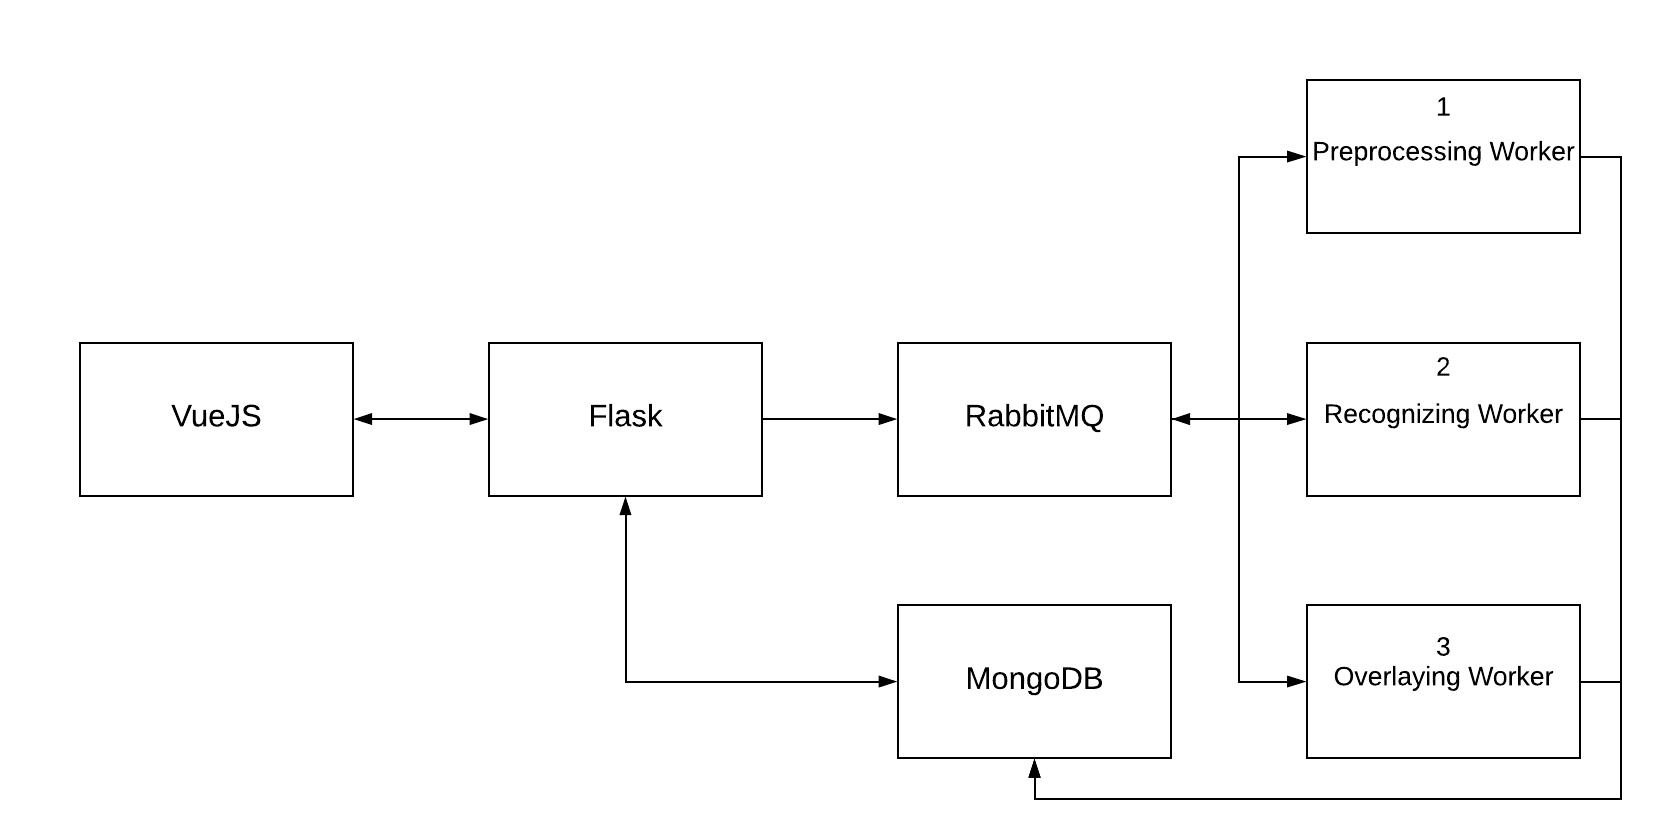
\includegraphics[width=1.0\linewidth]{images/overall-architecture}
 	\caption{Overall Architecture of the system}
 	\label{fig:overall-architecture}
 \end{figure}
 
 Figure 3.1 illustrate the flow of entire framework that implemented on the service. Vue.js is chosen as front-end, while back-end is built by using Flask. For the database, we decide to use MongoDB for storing the video information. For the process, we used RabbitMQ as task queue to send the tasks to a group of celery workers including pre-processing worker, recognizing worker and overlaying worker. The name of each worker indicates the job of that worker.
 
 \section{Front-end}
 In the front-end, there are only two pages, which are the upload video page and the video information page.
 On the upload page, users have to choose the video that they want to generate subtitle and select the recognizer before upload the video. Otherwise, the error message will appear on the page.
 %image
 \begin{figure}[H]
	\centering
	\captionsetup{justification=centering}
	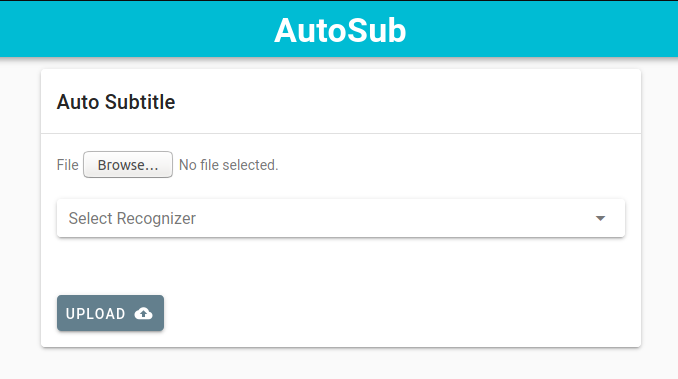
\includegraphics[width=0.8\linewidth]{images/main}
	\caption{Front-end main page}
	\label{fig:frontend-main}
 \end{figure}

\begin{figure}[H]
\centering
\captionsetup{justification=centering}
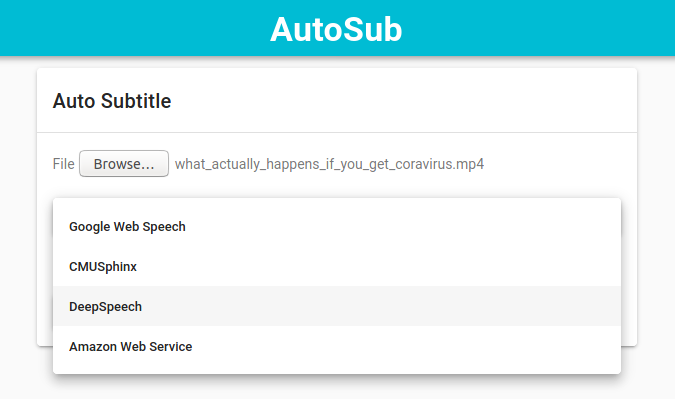
\includegraphics[width=0.8\linewidth]{images/main-with-options}
\caption{Available choices of speech recognition systems}
\label{fig:frontend-main-with-options}
\end{figure}
 
 On the video information page, it shows the video's id, filename and the status of the video. There are 5 kinds of statuses including `Video Uploaded', `Preprocessing Audio', `Recognizing Speeches', `Overlaying Video with subtitle' and `Completed'. Moreover, in this page, users allow to download two kinds of results, which are the generated subtitle file and overlayed video.
 %image
 \begin{figure}[H]
 	\centering
 	\captionsetup{justification=centering}
 	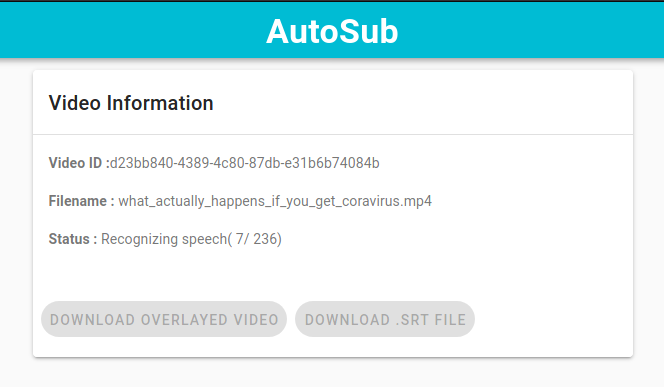
\includegraphics[width=0.8\linewidth]{images/info-recognizing}
 	\caption{The video information and status page}
 	\label{fig:frontend-info}
 \end{figure}

 \begin{figure}[H]
 	\centering
 	\captionsetup{justification=centering}
 	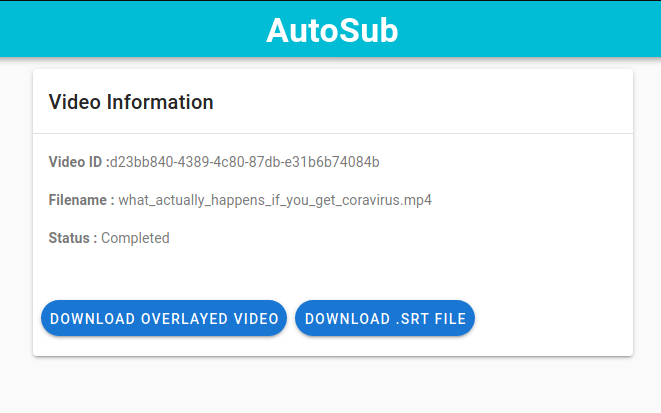
\includegraphics[width=0.8\linewidth]{images/info-completed}
 	\caption{The final look after the process is completed}
 	\label{fig:frontend-info-complete}
 \end{figure}
 
 \section{Database}
 The database design on this service is simple. The only data stored in database is the information of videos. This includes of id, filename, current status of the process, total amount of detected speech regions and the current number of recognized speeches.
 
 \section{Back-end API}
 There are the total of 4 APIs provided the communication between front-end and back-end server 
 \begin{itemize}
 	\setlength\itemsep{0em}
 	\item \textbf{/api/upload}: api for uploading video
 	\item \textbf{/api/get-status}: api for getting the information of video
 	\item \textbf{/api/get-srt}: api for downloading subtitle file
 	\item \textbf{/api/get-video}: api for downloading overlayed video
 \end{itemize}
 
 
 \section{Preprocessing Worker}
 In the preprocessing worker, the audio is processed by the steps in subsections. 
 However, unlike other speech recognition systems, Amazon Transcribe is an online paid service. It has different ways to process the audio, and our job is to upload the original video to the Amazon S3 bucket, and create the transcribe job.
 
 \subsection{Processioning Audio}
 There are some steps that required in this process. Since the input of the system is video, the first step in the process is to extract the audio from video. After that we need to convert the audio channels from stereo to mono by averaging the signal of left and right channels, and the last requirement is to resample the audio to 16000Hz.
 Filtering audio is one additional process to reduce the noise and non-speech regions of audio. In order to do this, we decided to use band-pass filter to filter out audio wave at human range fundamental frequency, which is around 85 to 255Hz with some extra padding\cite{nagaraja2019voiploc}.
 
 \subsection{Voice Activity Detection}
 After pre-processing the audio, the worker will detect the speech regions inside audio by using voice activation detection(VAD). Voice activity detection is a technique that use for distinguishing speech segments from background noise, and there are many ways to do it. The algorithm in this project is based on calculating the energy threshold. Firstly, we takes the sampling windows of the audio data and convert the values of sampling windows into energies using root mean square(RMS). Root mean square is the formula to calculate the average energy of the amplitudes. After getting an array of energies, we decided and calculate the cutoff percentile of energy to decide whether the windows are silence and speech. The last part in this algorithm is to loop over the sampling windows and find the speech segments by comparing the energy with the threshold.\cite{VADEnergybase}
 \begin{figure}[H]
 	\centering
 	\captionsetup{justification=centering}
 	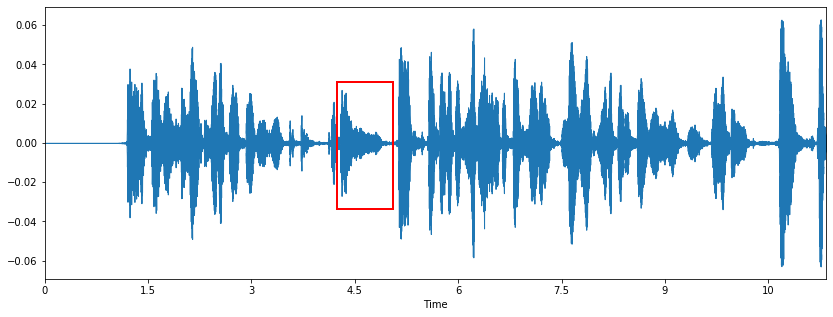
\includegraphics[width=0.9\linewidth]{images/vad}
 	\caption{Illustration of Voice Activity Detection}
 	\label{fig:vad}
 \end{figure}
 
 
 The drawback of this algorithm is that detected segments might be the background noise and music instead.
 
 After calculating the speech regions of the audio, we split the audio file into smaller chunks according to the audio segments.
 
 \section{Recognizing Worker}
 The main job of this worker is to recognize speeches from the audio chunks using the selected speech recognition system. Apart from the Amazon Transcribe, other three systems have the same flow. First, the worker read data from audio chunks and let the speech recognition recognize the audio. However, Some audio chunks are not speeches or recognizable resulting in errors, such as unknown value error and empty string. Thus, we need to reconstruct the sentences again base on the text and timing gap of each phrase.
 
 For the Amazon Transcribe, after create the transcribed job, the worker will wait until the job is complete and retrieve the json result that consist of words, punctuation and timestamps. Then, the worker construct the phrases based on them.
 
 The last step left in this worker is to generate the subtitle file by using the result we get.
 
 \section{Overlaying worker}
 The package that used to overlay the video is moviepy, a python module for video editing. The first step that the worker do is to load up the generated subtitle file from recognizing worker and the original video data. Then, moviepy read each phrase and timestamp of the subtitle and overlay on the original video. Overlaying video required a lot of memory usage, so rendering video with lower quality is an extra option. 
 
 % ------ Chapter 4 -------
 \chapter{Experiments and Results}
 The followings are automatic subtitle generation results of the sample videos and the accuracy evaluation of each automatic subtitle recognition system, which include of Amazon Transcribe, CMUSphinx, DeepSpeech and Google Web Speech. 

 \section{Result of Automatic Subtitle Generator}
 The screenshots that shown below come from the example video called `What Actually Happens If You Get Coronavirus?', which can be found in YouTube. The figures below are the examples of video that have the subtitles generated.
 
 \begin{figure}[H]
 	\centering
 	\captionsetup{justification=centering}
 	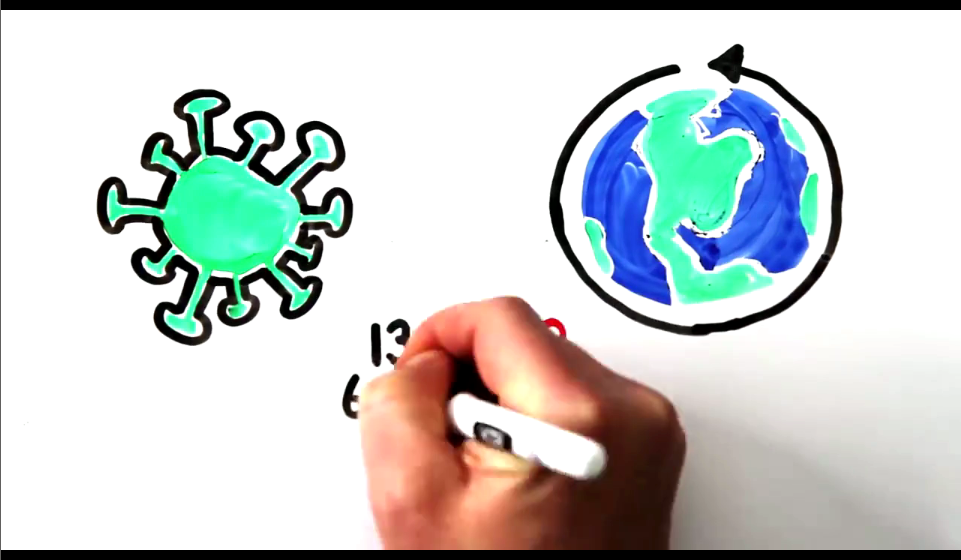
\includegraphics[width=0.7\linewidth]{images/example-video-original}
 	\caption{A screenshot from the example video}
 	\label{fig:example-vidoe-original}
 \end{figure}
 
 \begin{figure}[H]
 	\begin{minipage}{0.5\textwidth}
 		\centering
 		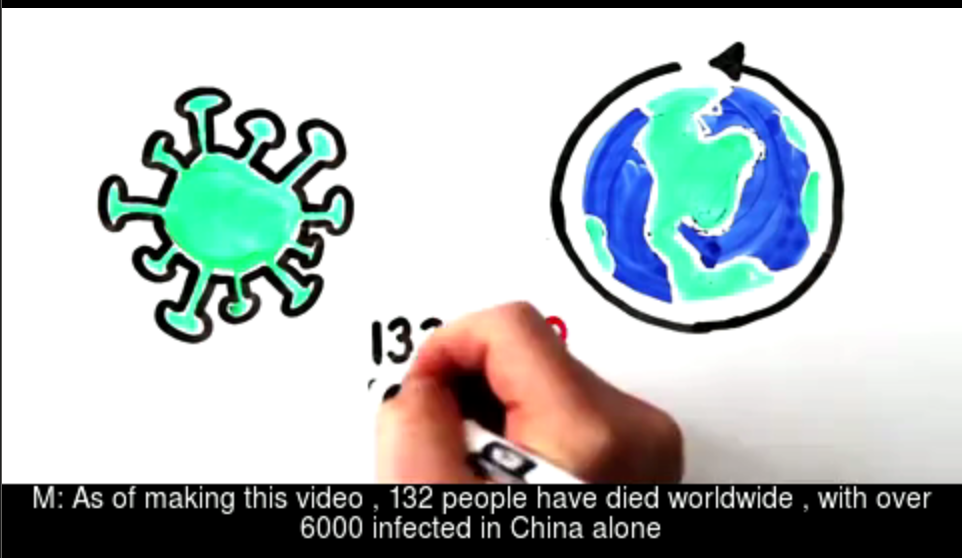
\includegraphics[width=0.9\textwidth]{images/example-video-aws} 
 		\captionof{figure}{Amazon Transcribe}
 		\label{fig:example-video-aws]}
 	\end{minipage}\hfill
 	\begin{minipage}{0.5\textwidth}
 		\centering
 		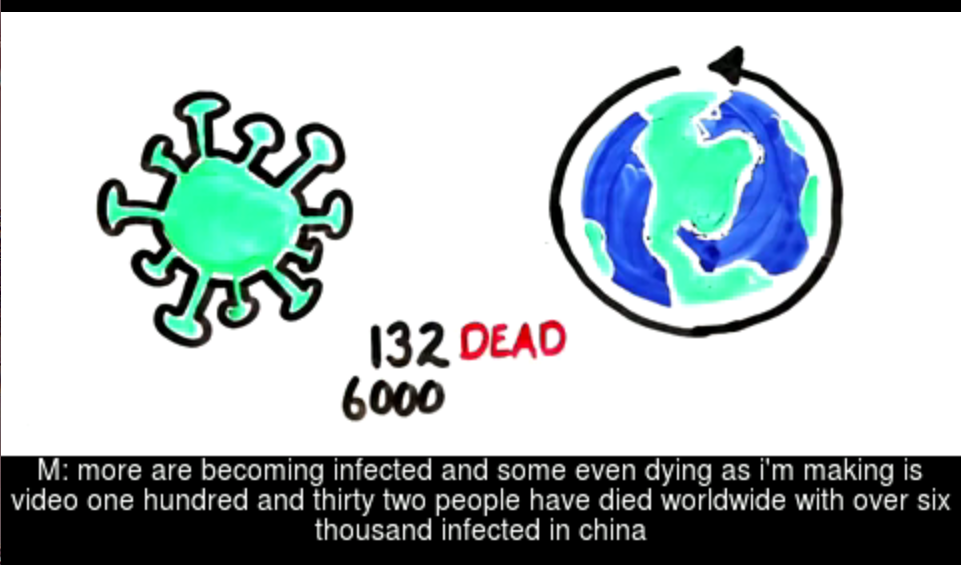
\includegraphics[width=0.9\textwidth]{images/example-video-cmusphinx} 
 		\captionof{figure}{CMUSphinx}
 		\label{fig:example-video-cmusphinx}
 	\end{minipage}
 \end{figure}
 
 \begin{figure}[H]
 	\centering
 	\begin{minipage}{0.5\textwidth}
 		\centering
 		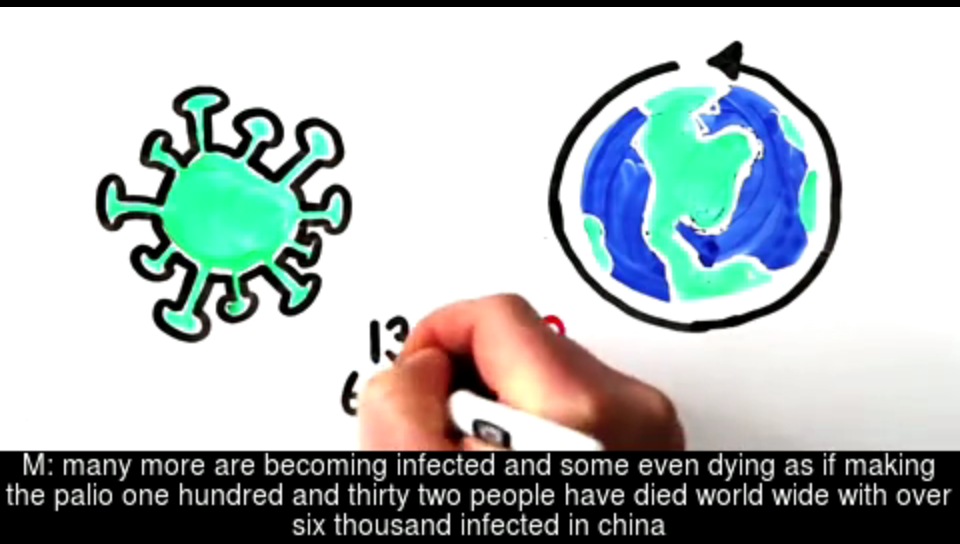
\includegraphics[width=0.9\textwidth]{images/example-video-ds} 
 		\captionof{figure}{DeepSpeech}
 		\label{fig:example-video-ds}
 	\end{minipage}\hfill
 	\begin{minipage}{0.5\textwidth}
 		\centering
 		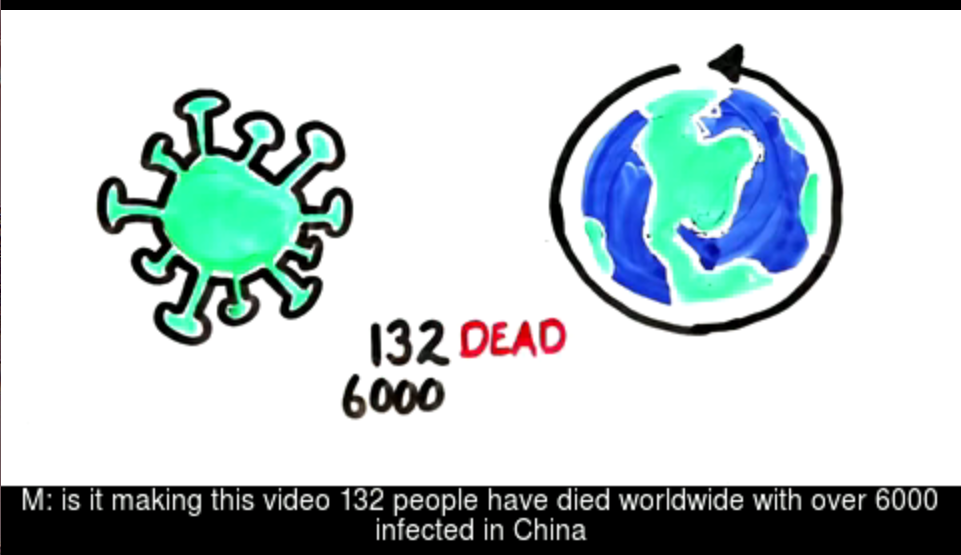
\includegraphics[width=0.9\textwidth]{images/example-video-gws} 
 		\captionof{figure}{Google Web Speech}
		\label{fig:example-video-gws}
 	\end{minipage}
 \end{figure}

 
 \section{Accuracy Evaluation}
 
 
 \subsection{Word Error Rate}
 Word error rate(WER) is a common metric that use to measure the performance of speech recognition and translation system. The lower word error rate is, the higher accuracy that the models can make. It is calculated by
 
 $$ WER = \frac{S+I+D}{N} $$
 
 S, I and D are stand for substitutions, insertions and deletions, respectively. They are the number of errors occurred in the speech recognition output. Substitutions are the text output that replaced the original text. Insertions are the extra words that speech recognition produced. Deletions are the words that were dropped from the original text. N is the total word count of the ground truth text.
 Before using word error rate, there are still some considerations need to be mention about. First, the word error rate excludes the punctuation in calculation. Second, word error doesn't tell the source of errors that occurred. Third, although word error rate can tell the performance of speech recognition system, it cannot fully tell the usability of the system.
 
 The below table show the list of videos that used in experiments and the WER results, and all of them can be searched on YouTube.
 
 \begin{center}
 	\begin{tabular}{ |c|c|c| } 
 		\hline
 		No. & Video Name & Type \\ 
 		\hline
 		1 & What Actually Happens If You Get Coronavirus? & Science\\
 		2 & Conversation Between Two Friends In English Speaking(Dialogue 1) & Dialogue \\
 		3 & Conversation Between Two Friends In English Speaking(Dialogue 2) & Dialogue \\
 		4 & Imaginary Numbers Are Real [Part 2: A Little History] & Math \\
 		5 & The Most Beautiful Equation in Math & Math \\
 		6 & Think Fast, Talk Smart: Communication Techniques(4 minutes) & Public Speaking \\
 		7 & What makes a good teacher great?(4 minutes) & Public Speaking\\
 		8 & Teaching Methods for Inspiring the Students of the Future(4 minutes) & Public Speaking \\
 		9 & Spider-Man: Into the Spider-Verse Trailer & Entertainment\\
 		10 & Joker Final Trailer (2019) & Entertainment \\
 		\hline
 	\end{tabular}
 \end{center}
 
 The box-plot on the figure below tells the word error rates that calculated from testing videos.
 \begin{figure}[H]
 	\centering
 	\captionsetup{justification=centering}
 	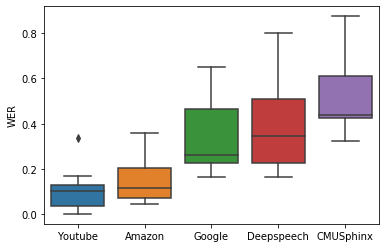
\includegraphics[width=0.7\linewidth]{images/boxplot}
 	\caption{A WER box-plot of testing videos}
 	\label{fig:wer-boxplot}
 \end{figure}
 According to the box-plot, YouTube has the lowest word error rate wcompared to others. The second is by Amazon Transcribe, and then followed by Google Web Speech, Deepspeech and CMUSphinx, respectively. 
 \section{Observations}
 This section is dedicated to discuss the reasons of why the performance of speech recognition system is low and will be categorized into four parts below
 \subsection{Name and Acronym}

 From the observations on text output, there are times that the speech recognition systems unable to recognize the words. The table below shows the examples of this error 
 \begin{center}
 	\begin{tabular}{ |c|c|c| } 
 		\hline
 		Speech Recognition System & Names & Acronym  \\ 
 		\hline
 		Ground truth & coronavirus & DNA or RNA\\
 		YouTube & coronavirus & DNA or RNA\\ 
 		Amazon Transcribe & corona virus & DNA or RNA\\
 		Google Web Speech & coronavirus & DNA or are\\
 		DeepSpeech & corona virus, cronies, crown virus &Diana or are\\
 		CMUSphinx & roto virus, throw the virus	& DNA of war are nay\\
 		\hline
 	\end{tabular}
 \end{center}
 
 As you can see in the table, DeepSpeech and CMUSphinx are clearly two of the speech recognition system that failed to recognize the word and produce sound-alike word instead. However, it is also because that the words `Coronavirus', `DNA' and `RNA' are the technical terms that people rarely talk about, so the pre-trained models are likely to focus more on the common speeches. Unlike other two, Youtube, Amazon Transcribe and Google Web Speech are large groups of providers and their target come from various groups of users, so their models are more adapt and keep updating.
 
 \subsection{Number}
 As we mentioned that the word error rate could not fully tell usability of the system, number is one of the example. The table below shows the examples of this issue.
 \begin{center}
 	\begin{tabular}{ |c|c|c| } 
 		\hline
 		Speech Recognition System & Example 1 \\ 
 		\hline
 		Ground truth & 132 people have died \\
 		YouTube & 132 people have died \\ 
 		Amazon Transcribe & 132 people have died \\
 		Google Web Speech & 132 people have died \\
 		DeepSpeech & one hundred and thirty two people have died \\
 		CMUSphinx & one hundred and thirty two people have died \\
 		\hline
 	\end{tabular}
 \end{center}
 \begin{center}
 	\begin{tabular}{ |c|c|c| } 
 		\hline
 		Speech Recognition System & Example 2 \\ 
 		\hline
 		Ground truth & \$1,\$2 and \$5\\
 		YouTube & \$1,\$2 and \$5\\ 
 		Amazon Transcribe & \$1.2 dollars and \$5\\
 		Google Web Speech & \$1,\$2 + \$5\\
 		DeepSpeech & one dollar two dollars and five dollars\\
 		CMUSphinx & one dollar dollars and five dollars\\
 		\hline
 	\end{tabular}
 \end{center}
 From the table, we can see that the outputs are understandable. However, if we look into the word error rate calculation, the number and symbol could be considered as errors instead.
 
 In the example 1, ground truth is `132 people have died'. the numerical character in text, 132, can also be read as `one hundred and thirty two', so from the users' perspective, they can understand both. However, in term of word error rate, this kind of result can effect its last value. For example, in the calculation, `132' is considered as one word, but on the other hand, `one hundred and thirty two' is considered as five error words. If we use `132' as the ground truth, the word error will be 5. This situation also applied to the example 2, where `\$1' is considered as one word while `one dollar' is considered as two words
 
 In terms of usability, both kinds are fine, but if the task requirement is numerical character, YouTube, Amazon Transcribe and Google Web Speech are the good choices. Even so, there are times that the engines recognize them as words, which also depend on the structure of sentences.
 
 
 \subsection{Accent, Pronunciation and Noise}
 Accent, pronunciation and noise are one of the main reason that cause the system unable to recognize the words or sentences. If the model isn't train for the particular accent and pronunciation, there is a high chance that accuracy of the speech recognition will be low and effect the word error rate.
 
 \begin{center}
 	\begin{tabular}{ |c|c| } 
 		\hline
 		Speech Recognition System & Example  \\ 
 		\hline
 		Ground truth & But what we will be looking at is how the corona virus actually.. \\
 		YouTube & But what we will be looking at is how the corona virus actually..\\ 
 		Amazon Transcribe & But what we will be looking at is how the corona virus actually \\
 		Google Web Speech & coronavirus Act \\
 		DeepSpeech & by that we will be looking at is how the crown a virus act actually \\
 		CMUSphinx & we will be looking at is how the krown virus\\
 		\hline
 	\end{tabular}
 \end{center}

 From the table above, the ground truth is `But what we will be looking at'. This phrase come from the video in YouTube called `What Actually Happens If You Get Coronavirus?' at 33 seconds of video. There are two speakers in videos, and this phrase is the transition between them. For this example, we will focus on the word, `But what'. At the start of this phrase, the speaker speak this word in a fast pace which cause some speech recognition engine unable to recognize the text. For example, DeepSpeech listen it as `by that', while Google Web Speeci API and CMUDSphinx unable to transcribe the beginning of sentence
 
 To give you another example, the table below shows the WER that calculated from the video in YouTube called Joker Final Trailer. As a movie trailer, the video has a lot noise and background music as well as the accent and pronunciation that different from normal video. 

 \begin{center}
 	\begin{tabular}{ |c|c| } 
 		\hline
 		Speech Recognition System & WER(\%)  \\ 
 		\hline
 		YouTube & $16.98\%$  \\ 
 		Amazon Transcribe & $22.64\%$  \\
 		Google Web Speech & $59.12\%$ \\
 		DeepSpeech & $79.87\%$\\
 		CMUSphinx & $87.42\%$ \\
 		\hline
 	\end{tabular}
 \end{center}

 As you can see, even the good speech recognition engine that YouTube used also has the high word error rate, and followed by Amazon Transcribe, Google Web Speech, DeepSpeech and CMUSphinx, respectively.
 
 \subsection{Systems Evalaution}
 In this subsection, we will give the pros and cons of that found in each speech recognition engines. 
 
 From the observations, it could be concluded the YouTube is the best one so far with the lowest word error rate even though sometimes, it failed to transcribe, especially on entertainment video.
 
 Amazon Transcribe won in second place. It has the low word error rate and come with punctuation, which help us to construct new phrases easily. Another good point is that it can detect the numerical character
 
 Google Web Speech API resulted in the third place. It could detect numerical characters like Amazon Transcribe, but sometimes, it could not identify the transition or short words of audio like `yes', `but' and `or.'
 
 DeepSpeech resulted in the fourth place in this competition, The main drawbacks are that it could not detect the name and acronym. Moreover, the pre-trained model is limit to American English, so sometimes, it could not predict other accent and pronunciation.
 
 CMUSphinx achieved the highest word error rate, and most of the cases, CMUSphinx predict the words that have the sound alike, but this doesn't mean that it cannot be use. The pre-trained model provided by CMUSphinx can do better in the videos that used lots of common words.
 
 Despite the fact of these results, the evaluation could be differ depend on the different configurations and settings.
 
 \section{Gender Recognition}
 \subsection{Dataset}
 We rely on the voice data provided by Kory Becker with the total amount of 3,168 records of males and females, and the data is pre-processed with 21 features.\cite{Dataset}
 \begin{itemize}
 	  \setlength\itemsep{0em}
 \item \textbf{meanfreq}: mean frequency (in kHz)
 \item \textbf{sd}: standard deviation of frequency
 \item \textbf{median}: median frequency (in kHz)
 \item \textbf{Q25}: first quantile (in kHz)
 \item \textbf{Q75}: third quantile (in kHz)
 \item \textbf{IQR}: interquantile range (in kHz)
 \item \textbf{skew}: skewness (see note in specprop description)
 \item \textbf{kurt}: kurtosis (see note in specprop description)
 \item \textbf{sp.ent}: spectral entropy
 \item \textbf{sfm}: spectral flatness
 \item \textbf{mode}: mode frequency
 \item \textbf{centroid}: frequency centroid (see specprop)
 \item \textbf{peakf}: peak frequency (frequency with highest energy)
 \item \textbf{meanfun}: average of fundamental frequency measured across acoustic signal
 \item \textbf{minfun}: minimum fundamental frequency measured across acoustic signal
 \item \textbf{maxfun}: maximum fundamental frequency measured across acoustic signal
 \item \textbf{meandom}: average of dominant frequency measured across acoustic signal
 \item \textbf{mindom}: minimum of dominant frequency measured across acoustic signal
 \item \textbf{maxdom}: maximum of dominant frequency measured across acoustic signal
 \item \textbf{dfrange}: range of dominant frequency measured across acoustic signal
 \item \textbf{modindx}: modulation index. Calculated as the accumulated absolute difference between adjacent measurements of fundamental frequencies divided by the frequency range
 label: male or female
 \end{itemize}
 \subsection{Result}
 For this project, gender recognition is an incomplete feature, and there are many improvement need to be done. To give you the brief information, the gender recognition models are trained by using the different methods, which are Support Vector Machine, K-Nearest Neighbor, Naive-Bayes and Random Forest. The cross-validation accuracy of the models are 98\%, 98\%, 89\%, and 97\%,respectively. However, they are overfitting and failed to generalize. This meaning that the models could not predict the gender. correctly The results are mostly go in one way either all males or all females.
 
 
  \bibliography{ref}
  \biography
  
\end{document}

